
%(BEGIN_QUESTION)
% Copyright 2010, Tony R. Kuphaldt, released under the Creative Commons Attribution License (v 1.0)
% This means you may do almost anything with this work of mine, so long as you give me proper credit

FOUNDATION Fieldbus H1 cable is comprised of two ungrounded conductors surrounded by a grounded shield.  Coupling devices provide easy connection points for new devices on the network segment:

$$\includegraphics[width=15.5cm]{i04575x01.eps}$$

\vskip 10pt

Suppose the H1 segment shown above is newly-constructed, and you are asked to perform some basic tests on the cable to ensure there are no major problems before it is energized for the first time.  Describe a simple way for you to electrically check for a {\it ground loop} in the trunk cable with as few steps as possible.

\vskip 20pt \vbox{\hrule \hbox{\strut \vrule{} {\bf Suggestions for Socratic discussion} \vrule} \hrule}

\begin{itemize}
\item{} Explain exactly why a ``ground loop'' is so problematic in a cable system.
\item{} Suppose an electrician wants to use a test instrument called a {\it megger} to check the integrity of a FOUNDATION Fieldbus H1 cable.  His plan is to check for ground faults as well as shorts between the cable conductors and/or between the conductors and the cable shield.  Do you agree with the electrician's plan?  Why or why not?
\item{} When the segment is up and running, may we use a handheld multimeter to measure Fieldbus signal strength, in lieu of an oscilloscope?  Why or why not?
\end{itemize}

\underbar{file i04575}
%(END_QUESTION)





%(BEGIN_ANSWER)

Hint: use an ohmmeter!

%(END_ANSWER)





%(BEGIN_NOTES)

Disconnect the shield ground at the host end of the cable, then measure resistance (ohms) between the disconnected shield wire and earth ground -- it should read open (ideally, infinite resistance).

%INDEX% Fieldbus, FOUNDATION (H1): segment troubleshooting

%(END_NOTES)

